
%% The first command in your LaTeX source must be the \documentclass command.
\documentclass[sigconf]{acmart}
\usepackage{scrextend}
\usepackage{float}
\addtokomafont{labelinglabel}{\sffamily\bfseries}

%%
%% \BibTeX command to typeset BibTeX logo in the docs
\AtBeginDocument{%
  \providecommand\BibTeX{{%
    \normalfont B\kern-0.5em{\scshape i\kern-0.25em b}\kern-0.8em\TeX}}}

\begin{document}
\title{Genetic Algorithms}
\maketitle
\section{Introduction}
Genetic Algorithms (GA) are a family of algorithms based on the theory of evolution. They derive the neighborhood, as well as the heuristics, for a local search by adhering to core concepts derived from nature. The three core concepts are
\begin{enumerate}
  \item Selection of the fittest 
  \item Crossover mating
  \item Random mutation
\end{enumerate}
There are many options when implementing a GA, but the core principles remain largely constant.

\section{General Procedure}
\subsection{Initialization}
The fundamental concept of a GA starts from a randomly selected population of DNA. Each DNA represents a solution to the problem and is composed of genes, with each gene representing a specific parameter in the solution. The population of DNA and succeeding generations of it act as the neighborhood in a local search

\subsection{Selection}
From the first core concept, the fittest DNA will be selected to pass their gene on to the next generation, in the hopes of preserving parameters that optimizes the fitness. Thus, from the initial population, the fitness of each DNA is evaluated, with the fitness function usually returning a value to be minimized or maximized. Common methods used to select a DNA based on its fitness include always selecting the highest fitness or using a probability distribution with weights proportional to the fitness.
An additional option at this stage is the inclusion of elitism. This sets a certain amount of fit DNA being automatically introduced into the next generation without any modification. This preserves the fittest DNA and guarantees that the next generation will have a lower bound of the fittest DNA. Thus, the algorithm always produces a solution that is better than or equal to the current one.

\subsection{Mating}
The second core concept of crossover mating works by allowing a child to inherit the fitter parameters from its parents. The method in which parameters are inherited is highly dependent on the requirements of the problem. This is repeated until the next generation of the population has been generated. 

\subsection{Mutation}
Each gene in a DNA has a chance to undergo mutation. When mutation occurs, a gene is replaced by another randomly generated gene. Similar to its application in the theory of evolution, mutation is used in a GA to introduce variation into the population. Thus, a GA can adapt to the situation and is less likely to be stuck at a local optimum as compared to other local search algorithms.

\subsection{Termination}
The steps from selection to mutation can be repeated for a fixed number of generations or until a certain cutoff time is reached. Even if multiple of the same solution is found in successive generations, there is no guarantee that optimal solution is found as the algorithm is reliant on random selection. The fittest DNA is then considered the optimal solution found by the algorithm.

\section{TSP Implementation}
\subsection{Terms}
For this implementation of TSP, we define the following terms can be defined as such
\begin{labeling}{Fitness\quad}
  \item[Gene] A set of x and y coordinates of a node 
  \item[DNA] A route that passes through each node only once and arrives back at the origin. This is a solution to TSP.
  \item[Fitness] The reciprocal of the tour length of a route. The shorter the router, the fitter the DNA.
\end{labeling}

\subsection{Methods}
The following methods have been chosen as the form of implementation at each stage.
\begin{labeling}{Termination\quad}
  \item[Selection] Each DNA is selected randomly, with the probability of selection being proportional to the relative fitness of the DNA among the population. The number of parents is fixed at 2 in this scenario to easily preserve the conditions a solution is required to have by TSP. 
  \item[Elitism] A percentage of the population with the fittest DNA are directly carried over to the next generation..
  \item[Crossover] A random segment, of half the length, of one parent is selected and forms the first half of the child. The remaining of half is comprised of the remaining genes in order of the other parent. This is done to ensure that no node is repeated in a DNA.
  \item[Mutation] If a gene undergoes mutation, another gene in the DNA is randomly selected and their places are swapped. This is done instead of simply picking a new gene to ensure that nodes are not repeated.
  \item[Termination] Upon termination, the fittest DNA will be the route with the shortest tour length found and is the most optimal solution produced by the algorithm.
\end{labeling}

\section{Pseudocode}
\section{Complexities}
\subsection{Time Complexity}
The time complexity for each generation can be calculated as follows
\begin{labeling}{Space for Next Generation\quad}
  \item[Initialization] O(N×Population Size)
  \item[Selection] O(N×Population Size)
  + O(Population Size log Population Size)
  \item[Mating] O(N×Population Size)
  \item[Mutation] O(N×Population Size)
  \item[Total Time Complexity] O(N×Population Size
  ×Number of Generations)
\end{labeling}
Thus, for a fixed set of hyperparameters,
\begin{labeling}{Space for Next Generation\quad}
  \item[Total Time Complexity] O(N)
\end{labeling}
This may seems fast, however, the constants, Population Size and Number of Generations, are usually very large and can easily dwarf the actual input size N. 
\subsection{Space Complexity}
\begin{labeling}{Space for Next Generation\quad}
  \item[Space for Population] O(N×Population Size)
  \item[Space for Next Generation] O(N×Population Size)
  \item[Total Space Complexity] O(N×Population Size)
\end{labeling}

\section{Design}
\subsection{Hyperparameters}
The following are hyperparameters that affect the optimal solution found.
\begin{labeling}{Number of Generations\quad}
  \item[Population Size] The amount of DNA in a pool available for mating. The larger the population, the higher the variation and the better the solution, but the longer it takes for an iteration of the algorithm. When the number of unique DNA in a population is equivalent to the possible number of solutions, GA is guaranteed to provide and optimum solution.
  \item[Elitism Factor] The proportion of the population’s fittest DNA being directly carried to the next generation without any modification. The higher the factor, the better fitter the population will when mating to produce the next generation. However, this reduces the variation and thus increases the probability of the solution only being a local optimum. When this factor is at 0, there is no guaranteed lower bound for the solutions and the optimal solution may decrease at each iteration.
  \item[Mutation Probability] The probability a gene might be mutated. The higher the probability, the higher the variation in the population. However, too high a probability prevents the child DNA from inheriting the fitter aspects from its parents. When the probability of mutation is 1, each child is completely random and does not inherit any parameters from its parents. This will perform worse than a brute force solution as the full solution space is explored at random with no guarantees of finding the actual optimum.
  \item[Number of Generations] With elitism, the higher the number of generations, the better the solution as the fittest DNA of each generation acts as the lower bound of the next. However, this increases the running time.
\end{labeling}

\subsection{Selection of Hyperparameters}
The hyperparameters are selected empirically. This is done by running the algorithm with different permutations of hyperparameters on a test dataset and selecting the parameters that consistently provide a low tour length. This has the drawback of selecting hyperparameters that might only be optimized for a certain dataset. Further extension to this can be choosing hyperparameters that are scaled to other heuristics such as the size of the dataset.
For this problem, the dataset from Atlanta was used as a test dataset as, due to its input size, it can reach a high level of quality in a reasonable amount of time. Datasets with smaller input size reach its optimum solution too quickly regardless of hyperparameters chosen and datasets with larger input size takes a much longer time to run and test. Each permutation was tested 3 times and the average time and tour length was used as the result.

\begin{figure}[h]
  \centering
  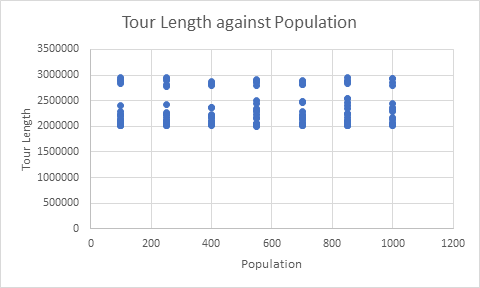
\includegraphics[width=\linewidth=]{genetic_pop_graph.png}
  \caption{Graph of Tour Length against Population Size for varying hyperparameters}
\end{figure}
\begin{figure}[h]
  \centering
  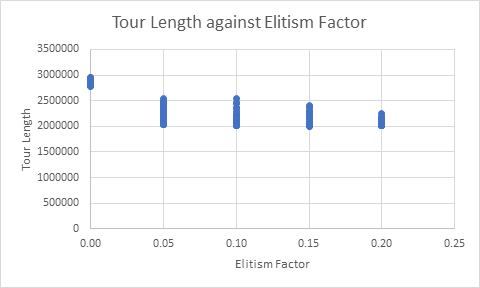
\includegraphics[width=\linewidth]{genetic_elite_graph.png}
  \caption{Graph of Tour Length against Elitism Factor for varying hyperparameters}
\end{figure}
\begin{figure}[h]
  \centering
  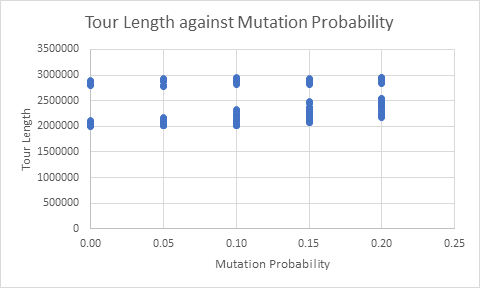
\includegraphics[width=\linewidth]{genetic_mutate_graph.png}
  \caption{Graph of Tour Length against Mutation Probability for varying hyperparameters}
\end{figure}

As can be seen from Figure 1, the effect of the population size on the variance of the solution length is negligible. A population of 250 was thus selected as it has the lowest mean. From Figure 2, an elitism factor of 0.2 was selected as it has the lowest variance. A mutation of 0.05 was selected instead of 0 even though the variance is slightly higher as to preserve the random nature of creating new neighborhoods for a local search. The number of generations was fixed at 10000 as the cutoff time serves as the termination condition.

\begin{table}
  \caption{Hyperparameters Selected}
  \label{tab:freq}
  \begin{tabular}{ccl}
    \toprule
    Parameter&Value\\
    \midrule
    Population Size & 250\\
    Elitism Factor & 0.2\\
    Mutation Probability & 0.05\\
    Number of Generations & 10000\\
  \bottomrule
\end{tabular}
\end{table}

\section{Theoretical Evaluation}
\subsection{Strengths and Weaknesses}
A GA is usually known for being able to quickly reach the vicinity of the optimum solution but takes a much longer time reaching the actual optimum. This is due to its probabilistic nature rather than a fixed heuristic. Most implantation of GA is used to reduce the solution space, before another algorithm is used to find the actual optimal solution. This is much akin to evolution, where specific evolutionary traits are determined randomly.

%%
%% The next two lines define the bibliography style to be used, and
%% the bibliography file.
\bibliographystyle{ACM-Reference-Format}


\end{document}
\endinput
%%
%% End of file `sample-authordraft.tex'.
